\chapter{ Экспериментальный раздел}
Результаты работы алгоритмов представлены на диаграммах изображенных на рисунках \ref{figure:bestCase}, \ref{figure:midCase} и \ref{figure:worstCase} на которых:

1 -- Сортировка простыми вставками(изображена черным цветом)

2 -- Сортировка слиянием(изображена красным цветов)

3 -- Сортировка пузырьком(изображена синим цветом)

\begin{figure}[ht!]
	\centering{ 
		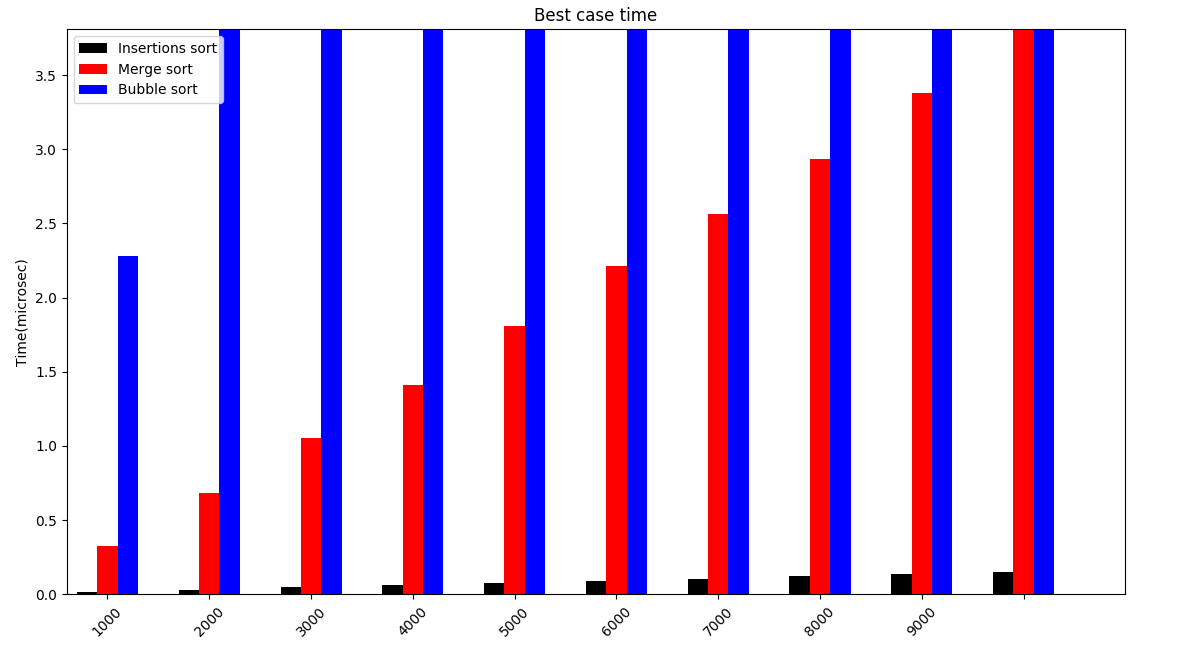
\includegraphics[width=1.1\textwidth]{img/bestCase.png}
        \caption{График, показывающий временные замеры алгоритмов сортировки для лучшего случая}\label{figure:bestCase}}
\end{figure}

\begin{figure}[ht!]
	\centering{ 
		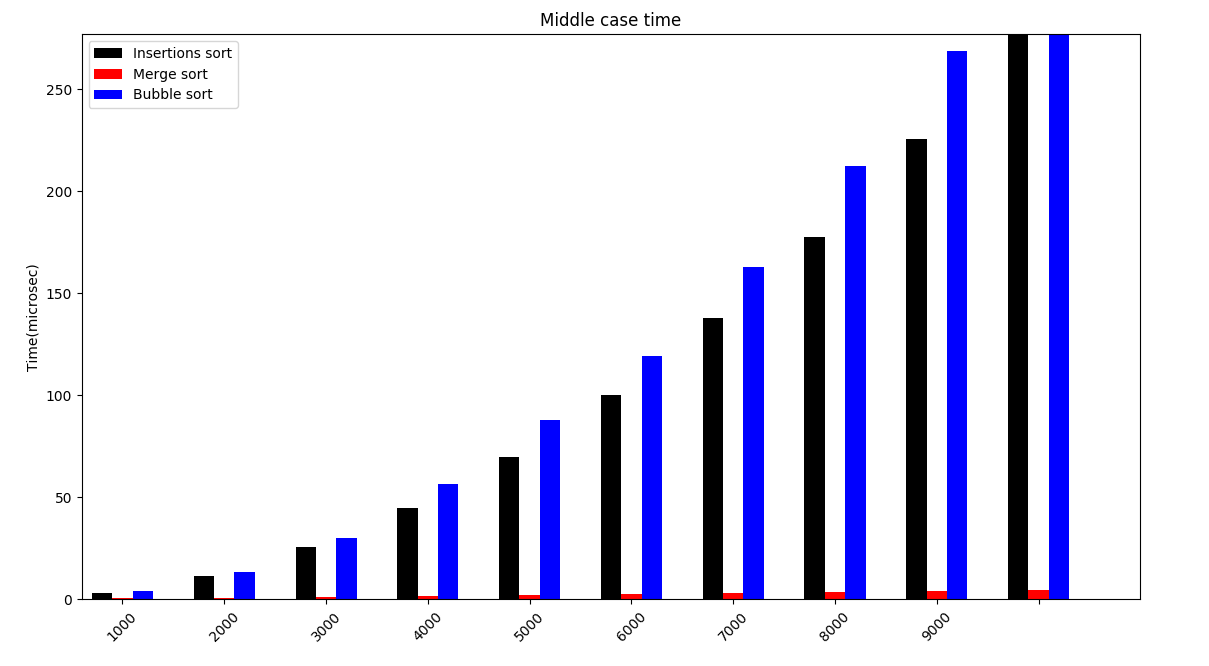
\includegraphics[width=1.1\textwidth]{img/midCase.png}
        \caption{График, показывающий временные замеры алгоритмов сортировки для произвольного случая}\label{figure:midCase}}
\end{figure}

\begin{figure}[ht!]
	\centering{ 
		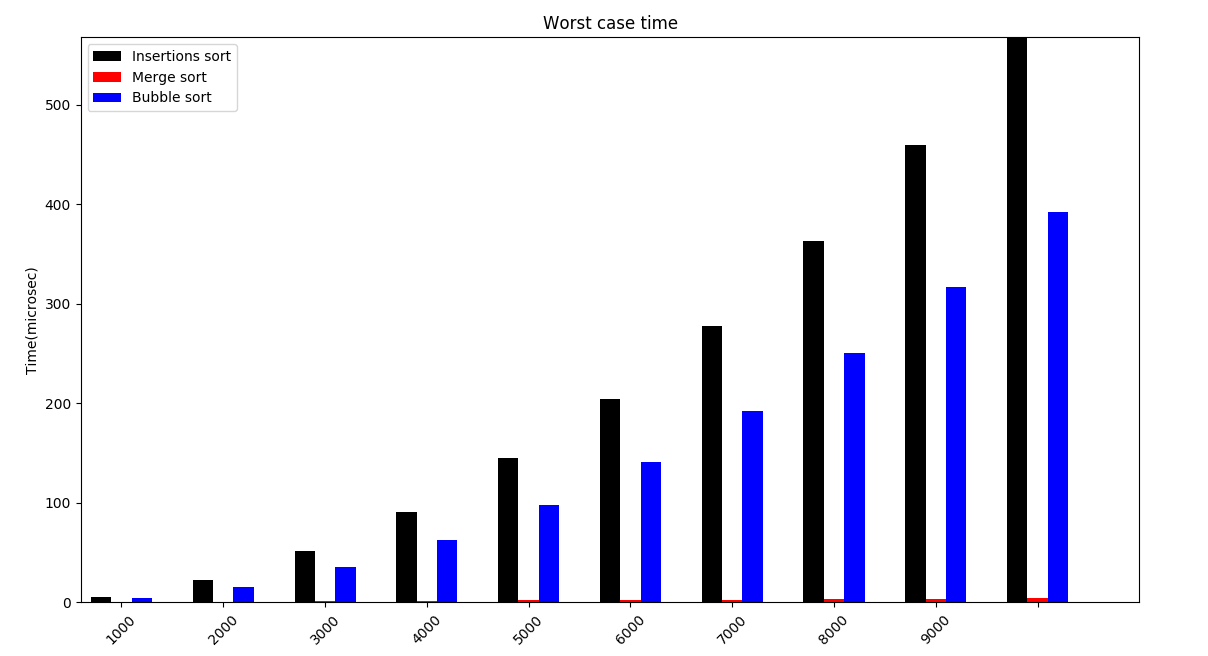
\includegraphics[width=1.1\textwidth]{img/worstCase.png}
        \caption{График, показывающий временные замеры алгоритмов сортировки для худшего случая}\label{figure:worstCase}}
\end{figure}


По полученным данным можно сделать вывод, что стандартный алгоритм перемножения матриц работает медленнее, чем классический алгоритм Винограда и улучшенный алгоритм Винограда. Улучшенный алгоритм работает быстрее по времени, чем классический. Если обратиться к рассчитанным трудоемкостям алгоритмов, можно заметить, что стандартный алгоритм менее трудоемкий, чем два других, но время, затрачиваемое на рассчет матрицы стандартным методом все равно очень большое. Так как это зависит от модели вычислений, где умножение и обращения к индексам и сложение были взяты за 1, можно сказать, что следует учитывать некоторые ньюансы при выборе весов операций, чтобы вычесленная трудоемкость была более точной.
